\section{Workflow Overview}

The general methodology for this work is described in figure
\ref{fig:workflow}. Technical portions of figure \ref{fig:workflow}
are discussed in the following sections.

\begin{figure}
  \centering
  \makebox[0pt]{
    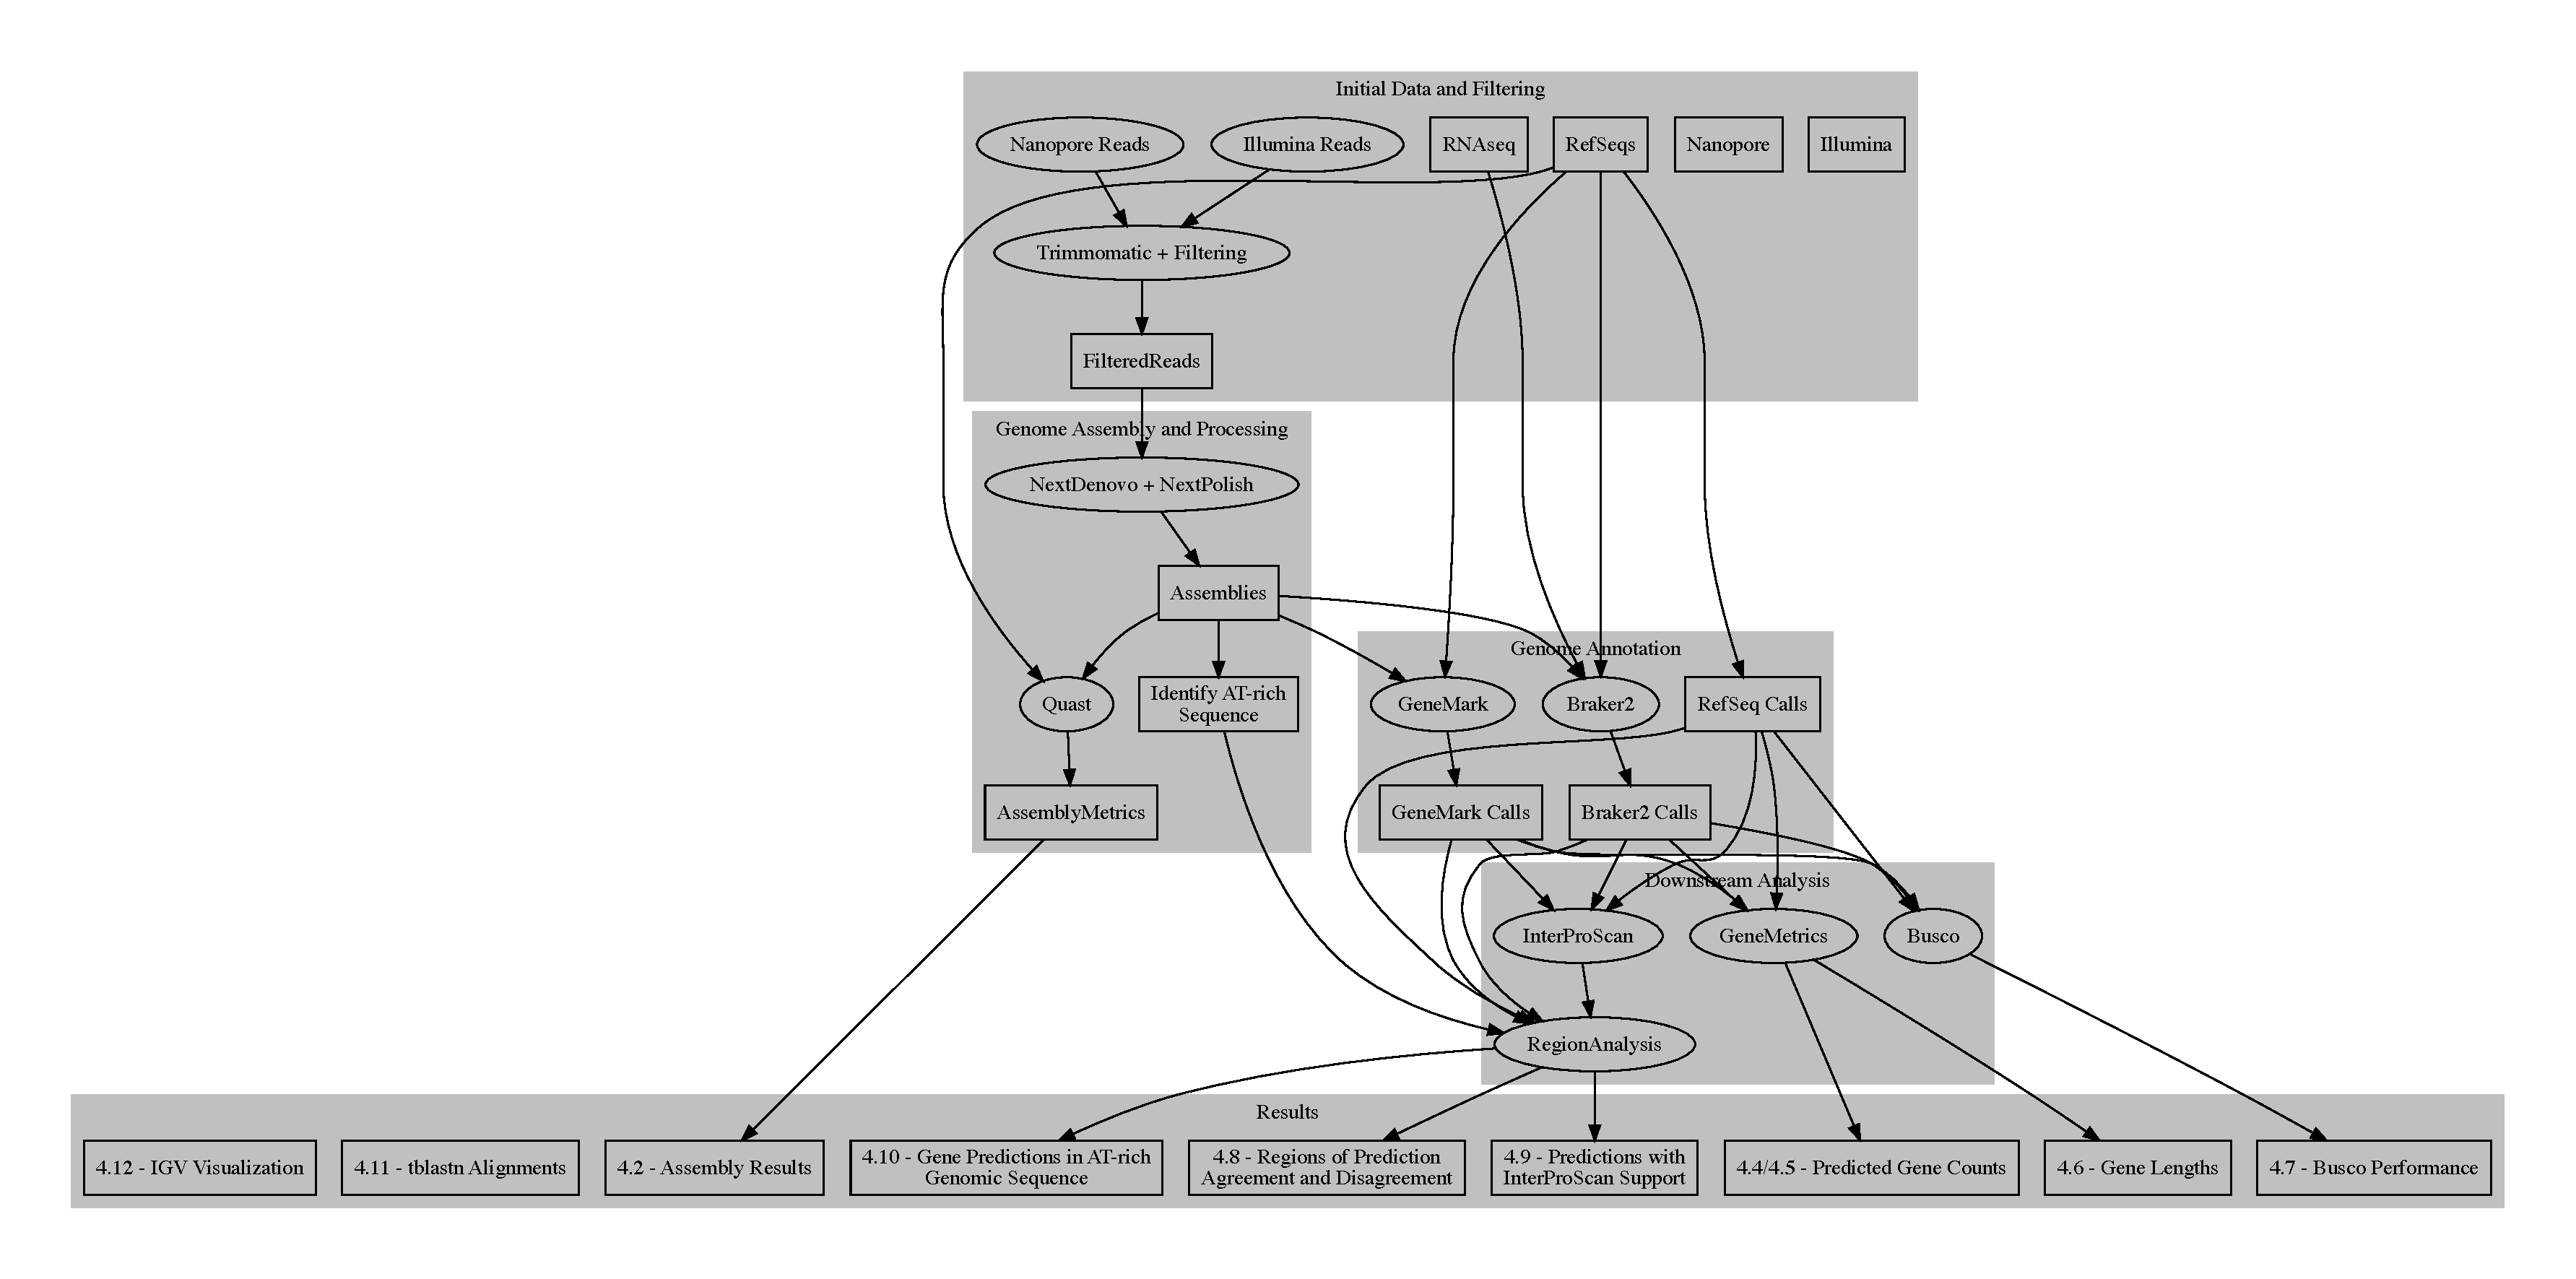
\includegraphics[width=1.25\textwidth]{./figures/data-flowchart.pdf}
  }
  \caption{A flowchart of the methodology followed in this
    research. The workflow is broken up into sections based on the
    processes and data involved at each step. Oval-shaped nodes
    represent steps involved in the processing of data, while
    rectangular nodes represent intermediate datasets and results.}
  \label{fig:workflow}
\end{figure}


\section{Sequence Pre-processing and Assembly}

% somewhere here...
% The training was performed using roughly 145 million Illumina
% paired end RNAseq reads on the \textit{Trichoderma reesei} genome.

Genomic sequences were generated for DC1 and Tsth20 using
Nanopore\cite{Wang2021} and Illumina\cite{Bennett2004} sequencing
technologies. Nanopore data was not processed prior to
assembly. Illumina sequencing data was filtered using Trimmomatic
v0.38\cite{Bolger2014} with filtering criteria as follows:
SLIDINGWINDOW:4:28, LEADING:28, TRAILING:28, MINLEN:75. Only surviving
paired-end reads were used for further analysis.

Genomic Nanopore sequences from DC1 and Tsth20 were assembled in to
contigs using NextDenovo\cite{Hu2024} v2.5.0 and then polished with
Illumina sequences using NextPolish\cite{Hu2020} v1.4.1. Assembly and
polishing were both performed using default parameters. Final assembly
metrics were calculated using QUAST v5.0.2\cite{Gurevich2013} with
default parameters.

%In an attempt to produce high quality assemblies of DC1 and Tsth20, We
%decided on a set of tools named NextDenovo and NextPolish as they have
%produced excellent assemblies based on previous experience. (should
%find a citation to confirm this)

%(Might be better for discussion or omitted since it is specific to our
%setup) Initial attempts to run the example dataset resulted in
%permissions errors due to the management of the storage system being
%used, which were encountered with other tools in the past. To remedy
%this, the software installation was copied to RSMI's scratch space on
%Copernicus. Once the approriate permissions were given to run
%nextDenovo, the example dataset was run without issue.

%Following assembly using nextDenovo, Illumina sequence data from DC1
%and Tsth20 was used to polish each respective genome using
%nextPolish. Default parameters were used from assembly except for
%modification of the parallel option to reduce processing times.

%\subsection{Repeat Masking}

%In order to evaluate the performance of gene finding tools in
%repetitive or low complexity regions in the context of
%\textit{Trichoderma} genomes, we must first identify said regions in
%the genomes considered. To do this, the GenericRepeatFinder tool was
%used, which is a \textit{de novo} repeat detection tool
%\cite{10.1104/pp.19.00386}. GenerifRepeatFinder detects three
%different types of repeats, those being MITEs, TDRs and TIRs. Commands
%used for this program follow the example commands provided on the
%GitHub page for the GenericRepeatFinder project.

\section{Gene Prediction Using GeneMark-ES}

\textit{Ab initio} gene finding was performed using GeneMark-ES
v4.71\cite{Borodovsky2011}. Default parameters were used in all cases
except for the fungal option, which was allowed the use of a GeneMark
model specific to fungal genomes.

%General command structure for GeneMark-ES:
%
%gmes\_petap.pl --ES --fungus
%--format gff3 --cores 48 --sequence /path/to/sequence

\section{Gene Prediction Using Braker2}
\label{met:braker2}

For evidence-based gene finding, Braker2 v3.0.2\cite{Bruna2021} was
used with \textit{Trichoderma reesei} selected as the reference
organism for training. RNAseq datasets from \textit{T. reesei} were
downloaded from the NCBI short-read archive using the
sra-toolkit\cite{NCBI2025} and were not trimmed or filtered prior to
their use in Braker2 training. Default parameters were used to train a
Braker2 model on \textit{Trichoderma reesei} data except in the case
of the fungal option, which was used for this analysis for improved
gene-finding performance in fungi. The trained Braker2
\textit{T. reesei} prediction model was then applied to all assemblies
with default parameters.

Braker2 also provides a UTR option to predict upstream sequence
features, but that option is experimental and was left off for this
work.

%The variables that need to be set are AUGUSTUS\_CONFIG\_PATH and
%TSEBRA\_PATH. Augustus, by defuault, tries to write species
%information to the location where the software is installed. In this
%case, we don'thave write permissions to the compute canada software
%stack hosted byt Research Computing, so the AUGUSTUS\_CONFIG\_PATH
%variable must be set in order to create a writeable directory. As long
%as that path has a directory within it called braker, and a species
%directory within the braker directory, things should go
%smoothly. TSEBRA is a set of scripts also made by the creators of
%Braker and is required to merge results from the various gene
%prediction tools involved in the Braker2 pipeline. The TSEBRA\_PATH
%simply points to the directory where TSEBRA is located Both Braker2
%and TSEBRA can be cloned directly from GitHub (links to come)

\section{Binomial Tests on CDS Lengths}

In section \ref{section:lengths}, the coding DNA sequences (CDS) of
predicted genes were tested using a binomial test, under the null
hypothesis that the probability of a gene being in normal or AT-rich
genomic sequence is proportional to the total lengths of normal or
AT-rich sequence in the assembly.

\section{Evaluating Gene-Finder Performance Using BUSCO}

To assess the general performance of gene-finders, BUSCO
v5.7.1\cite{10.1093/bioinformatics/btv351} was selected as a tool to
determine a gene-finder's ability to predict a set of conserved
ortholagous genes. The BUSCO Metaeuk pipeline was run using the BUSCO
fungi\_Odb10 fungal lineage dataset to capture highly conserved genes
in fungal genomes. This pipeline was applied to all genome assemblies
used in this work. (note for us to discuss: I used transcriptome
mode...)

\section{Region Identification Procedure}
\label{section:region-met}

Predictions and results from previous steps were then processed into
overlapping regions of predictions and annotations. A region is
defined as a set of start and stop genomic coordinates which contains
one or more overlapping feature. We also define a feature as a set of
start and stop positions associated with a single gene prediction,
annotation or other data point of interest.

Overlapping features were processed into regions using a concept
similar to Allen's interval algebra\cite{DECHTER2003333}. The
algorithm first sorts all features on each contig by start coordinate
and then iterates over each feature, identifying overlaps with
previous features to identify regions of overlapping
features. Pseudocode for the algorithm is shown in algorithm
\ref{alg:regions}. This processing was performed with Python
v3.12.4\cite{Foundation} and the GFF package from BCBio\cite{Chapman}
for easy GFF parsing.  The resulting regions are then further
processed to identify trends and behaviours of gene finders in the
context of other annotated information and features.

\begin{algorithm}
  \begin{algorithmic}
    \State INPUT:\ list\ of\ GFF\ files,\ $GFFList$
    \State RETURNS:\ list\ of\ regions,\ $regionList$
    \For{\texttt{<each GFF in GFFList>}}
    \State $allFeatures \gets GFF.features$
    \EndFor
    \State $sortedFeatures \gets sortStartCoord(allFeatures)$
    \State $regionList \gets []$
    \For{\texttt{<each feature in sortedFeatures>}}
      \If{$feature = firstFeature$}
        \State $currentRegion \gets newRegion$
        \State $currentRegion.start \gets feature.start$
        \State $currentRegion.end \gets feature.end$
      \ElsIf{$feature = lastFeature$}
        \State $regionList \gets region$
        \State $return\ regionList$
      \ElsIf{$feature\ overlaps\ currentRegion$}
        \State $currentRegion \gets updateStartStopPositions$
        \State $currentRegion \gets feature$
      \Else
        \State $regionList \gets currentRegion$
        \State $currentRegion \gets newRegion$
        \State $currentRegion \gets feature.start$
        \State $currentRegion \gets feature.end$
      \EndIf
    \EndFor
    \State $return\ regionList$
  \end{algorithmic}
  \caption{the general algorithm underlying the region identification
    process.}
  \label{alg:regions}
\end{algorithm}

\section{Functional Annotation Using InterProScan}

The predicted proteins from each gene finder were functionally
annotated using InterProScan
v5.65-97.0\cite{10.1093/bioinformatics/btu031} without the match
lookup service and with the following analyses included: AntiFam-7.0,
CDD-3.20, Coils-2.2.1, FunFam-4.3.0, Gene3D-4.3.0, Hamap-2023\_01,
MobiDBLite-2.0, NCBIfam-13.0, PANTHER-18.0, Pfam-36.0, PIRSF-3.10,
PIRSR-2023\_05, PRINTS-42.0, ProSitePatterns-2022\_05,
ProSiteProfiles-2022\_05, SFLD-4, SMART-9.0,
SUPERFAMILY-1.75. InterProScan was run on all predicted proteins using
default parameters. The resulting protein annotations were mapped back
to the gene predictions and processed using the region identification
algorithm in section \ref{section:region-met}.

\section{Identification of AT-rich Genomic Windows}

Sliding windows of GC content over each \textit{Trichoderma} assembly
were calculated using isochore from the EMBOSS tool suite
v6.6.0\cite{Rice2000}. The sliding window used was 250bp wide with a
50bp shift. A window was classified as AT-rich if the sequence
contained lower than 28\% GC content. The genomic sequences from
AT-rich windows were mapped to a GFF file and processed using the
region identification algorithm described in section
\ref{section:region-met}.

\section{Ground-truthing with BLAST}

Need to flesh this out if I write results section.

\section{Visualization of Identified Regions}

Results from the region identification process were visualized using
the IGV genome browser v2.19.1\cite{Robinson2011}.

%=======
%Example command for braker2:
%
%/scratch/p2irc/p2irc\_rsmi/cbe453/masters/software/braker2/BRAKER/scripts/braker.pl
%--gff3 --threads 60
%--TSEBRA\_PATH=/scratch/p2irc/p2irc\_rsmi/cbe453/masters/software/braker2/tsebra/TSEBRA/bin/
%--genome /path/to/sequence --species=TreeseiFungal --fungus
%--useexisting
%
%BUSCO methodology (from research questions)
%The BUSCO method was applied using two BUSCO subsets,
%one generally applicable for fungi, and another targeting an
%evolutionary branch more closely related to \textit{Trichoderma}.
%
%Stats for length analysis (from research questions)
%The first statistical tool to be applied is ANOVA (analysis of
%variance) to compare the mean lengths genes predicted by each gene
%finding tool with the null hypothesis being that the mean of predicted
%gene lengths should be the same across all tools considered. In
%addition to ANOVA, pairwise comparisons of the distributions using a
%Kolmogorov–Smirnov test is appropriate. The null hypothesis in this
%test would be that the gene lengths are sample from the same
%distribution.
%
%Stats for binomial tests (from research questions)
%To do this, a binomial test will be used, with the null hypothesis
%being that the number of genes predicted in regions of normal and
%abnormal GC content should be proportional to the length of normal and
%abnormal GC content regions in the assembly. For example, if 30
%percent of the genome is comprised of anomalous GC content, then we
%would expect 30 percent of predicted genes to be present in those
%regions. In addition to anomalous GC content, this test can be applied
%to repetitive content in assemblies as well.
%
%Stats for regions (from research questions)
%From these results, Venn diagrams will be generated with
%Jaccard index calculated for each combination of gene finding
%tools. The region identification process can also be extended to
%include features identified by other tools, such as BLAST hits to
%validated gene models from other organisms and small RNAs. Chi2
%goodness of fit tests can then be applied to counts of 'validated'
%gene predictions or other features with the same null hypothesis that
%gene finders should predict the same number of features.
